\pdfoutput=1

\documentclass[11pt,DIV=16,parskip=half]{scrartcl}
\usepackage{algorithm,algorithmic}
\usepackage{amsmath,amssymb,amsfonts}
\usepackage{graphicx}
\usepackage{hyperref}
\usepackage{multirow}
\usepackage{svg}
\usepackage{textcomp}
\usepackage[svgnames]{xcolor}
\usepackage{tikz}
\usetikzlibrary{shapes.geometric, positioning, arrows, arrows.meta, decorations, decorations.pathmorphing, backgrounds, fit, petri, chains}

\tikzset{
	component/.style={
		font=\small\itshape,
text width = 2cm},
	group/.style={
		draw=gray!40,
		dashed,
		decoration={zigzag,
		amplitude=0.5}
	},
	outline/.style={
		draw=black!50,
		inner sep=5pt,
		decorate,
		decoration={random steps,
		segment length=10pt,
		amplitude=1pt}
	},
	wip/.style={
		minimum height=1cm,
		minimum width= 2cm,
		dashed,
		rounded corners=2pt,
		draw=gray!80,
		fill=LightCoral!30
	},
	existing/.style={
		minimum height=1cm,
		minimum width= 2cm,
		rounded corners=2pt,
		draw=gray!80,
		fill=gray!20
	},
	flowWip/.style={
		draw=gray!80,
		dashed,
		-Stealth},
	flowExisting/.style={
		draw=gray!80,
		-Stealth
	},
}


\usepackage[backend=biber, bibencoding=utf8, giveninits=true,
maxbibnames=99, % show all authors in the bibliography
maxalphanames=1, minalphanames=1, style=ieee, backref=false]{biblatex}
% Sets the bib file
\addbibresource{refs.bib}

% Basic information
\title{Verification in Open-Source Hardware Design Tools}
\author{Tobias Wölfel, \href{mailto:tobias.woelfel@hm.edu}{tobias.woelfel@hm.edu}}
\date{December 2024}

\begin{document}
\maketitle

\section{Introduction}
With the increasing complexity of hardware architectures, the need for verification
is becoming more important and demanding. One possibility to verify hardware
description is to specify timing properties which are later checked.

One way to specify such properties is to use linear temporal logic (LTL).
The support for LTL is very limited in open-source design tools. One central
tool to connect different steps in hardware design flow is \textit{Circuit IR
Compilers and Tools (CIRCT)}.

By adding LTL support to CIRCT and a contiuous flow between differnt tools,
more capable verification will be possible. With more information available at
a central location, research can concentrate on how to leverage those insights.
Additionally, with transformations into other steps in the design process, this
can allow for new and faster ways for verification.

An application to verify the integrity of a system is a RISC-V core.
With an enhanced verificaion of the core, the trust to the working of the
implemention is not changed when adding new features with RISC-V extentions.


\section{Related Work}
Describe the related work and state of the art.
Try to find a balance between covering relevant approaches and detailing those lines of work which are closest to your planned contribution.

Limit yourself to about 300 words, try to avoid references of questionable quality (websites, unverified arxiv preprints, ...) and make sure your references are formatted correctly, e.g.~\cite{cooley1965-fft}.

% - LTL support in Chisel, higher abstraction, greater need to verify the lower levels
% - SystemVerilog Assertions and support in open source tools
% - What can be done with LTL?



\section{Thesis Objective}
Based on the related work, identify the research gap you will be addressing.
Try to formulate research questions that your thesis will answer.
Describe the overall expected outcome of your research.
Helpful formulations could be as below

Consider this an executive summary and limit yourself to 150 words.

The objective of this thesis is ...

To achieve this goal, the following main research questions must be addressed: ....

% Formal verification
% FPGA testing
% unbounded vs bounded model checking (state explosion)


\section{Research Outline}
Sketch an outline of your research.
What problems will be addressed, how will you solve them?
What are data or infrastructure requirements, and how will you meet them?
How do you measure progress and success in your research?
You can think of this as work packages or milestones that you describe.
Briefly argue why your research will lead to a Dr.-Ing. or Dr. rer. nat.

Limit yourself to about 500 words, use figures, schemes, tables or itemized formatting as needed.

% - in which way can LTL be used for extentions, is there a way to automate property specifications?
% - How can LTL be used for formal verification?
% - Which insights into a hardware design can be deduced from the specified properties and sequences?

\begin{figure}[htb]
\centering
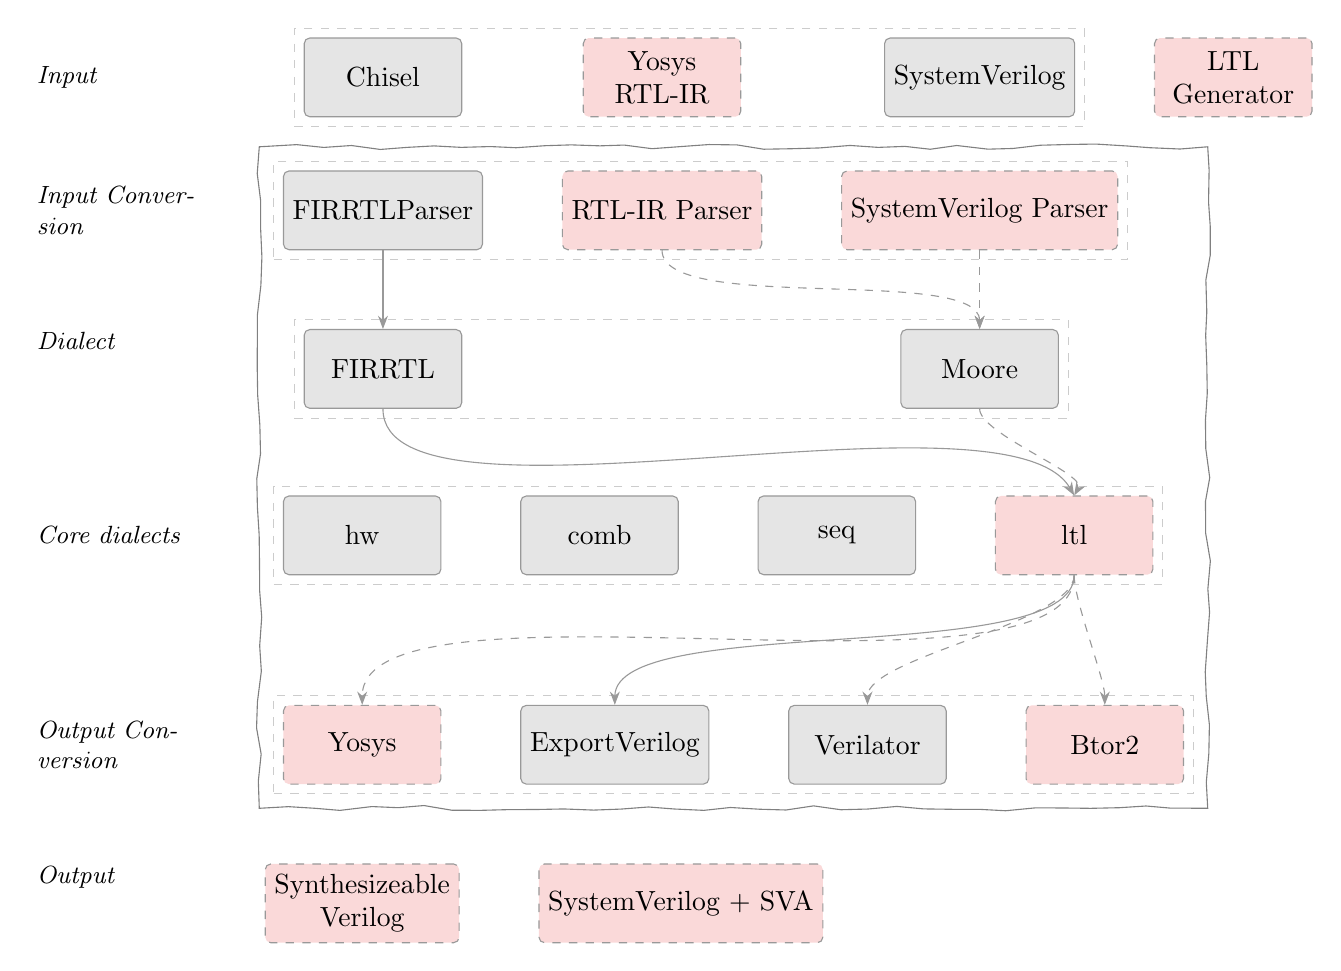
\begin{tikzpicture}
	% input languages
	\node [component] (inputLanguages) {Input};
	% input conversion
	\node [component, below=of inputLanguages] (inputConversion) {Input Conversion};
	\node [existing, right=of inputConversion] (firrtlParser) {FIRRTLParser};
	\node [wip, right=of firrtlParser] (yosysParser) {RTL-IR Parser};
	\node [wip, right=of yosysParser] (slang) {SystemVerilog Parser};
	\node [group, fit=(firrtlParser) (yosysParser) (slang)] (inputConversionBbox) {};

	% input languages (cont. with alignment to input conversion)
	\node [existing] at (firrtlParser|-inputLanguages) (chisel) {Chisel};
	\node [wip, align=center] at (yosysParser|-inputLanguages) (yosysrtl) {Yosys\\RTL-IR};
	\node [existing] at (slang|-inputLanguages) (sv) {SystemVerilog};
	\node [wip, right=of sv, align=center] (ltlgen) {LTL\\Generator};
	\node [group, fit=(yosysrtl) (sv) (chisel) (yosysrtl) (sv)] (inputR) {};

	% Dialects
	\node [component,below=of inputConversion] (dialects) {Dialect};
	\node [existing, below=of firrtlParser] (firrtl) {FIRRTL};
	\node [existing, below=of slang] (moore) {Moore};
	\node [group, fit=(firrtl) (moore)] (dialectsR) {};

	% core dialects
	\node [component,below=2cm of dialects] (coreText) {Core dialects};
	\node [existing, right=of coreText] (hw) {hw};
	\node [existing, right=of hw] (comb) {comb};
	\node [existing, right=of comb] (seq) {seq};
	\node [wip, right=of seq] (ltl) {ltl};
	\node [group, fit=(hw) (comb) (seq) (ltl)] (coreR) {};

	% output conversion
	\node [component,below=2cm of coreText] (outputConversion) {Output Conversion};
	\node [wip, right=of outputConversion] (yosys) {Yosys};
	\node [existing, right=of yosys] (exportVerilog) {ExportVerilog};
	\node [existing, right=of exportVerilog] (verilator) {Verilator};
	\node [wip, right=of verilator] (btor2) {Btor2};
	\node [group, fit=(yosys) (exportVerilog) (verilator) (btor2)] (outputConversionBbox) {};

	% CIRCT
	\node [outline, fit=(inputConversionBbox) (coreR) (outputConversionBbox)] (circt) {};

	% Output Language
	\node [component, below=of outputConversion] (outputLanguages) {Output};
	\node [wip, below=of yosys, align=center] (verilog) {Synthesizeable\\ Verilog};
	\node [wip, right=of verilog, align=center] (verilog) {SystemVerilog + SVA};

	% Connect input conversion to dialects
	\draw [flowWip] (yosysParser.south) to [out=-90, in=90, looseness=0.5] (moore.north);
	\draw [flowWip] (slang) -- (moore.north);
	\draw [flowExisting] (firrtlParser) -- (firrtl);

	% Connect dialects to core
	\draw [flowExisting] (firrtl.south) to [out=-90, in=120, looseness=0.5] (ltl.north);
	\draw [flowWip] (moore.south) to [out=-90, in=60, looseness=0.5] (ltl.north);

	% Ltl to all output conversions
	\draw [flowWip] (ltl) to [out=-90, in=90, looseness=0.5] (yosys);
	\draw [flowExisting] (ltl) to [out=-90, in=90, looseness=0.5] (exportVerilog);
	\draw [flowWip] (ltl) to [out=-90, in=90, looseness=0.5] (verilator);
	\draw [flowWip] (ltl) to [out=-90, in=90, looseness=0.5] (btor2);
\end{tikzpicture}
	\caption{LTL dialect as a central component in enabling verification support across a wide range of open source EDA tools.}
	\label{fig:toolOverview}
\end{figure}

\printbibliography

\end{document}
